\documentclass[aps,prd,superscriptaddress,nofootinbib,floatfix,10pt]{revtex4-2}

\usepackage{amsmath,amssymb,amsthm}
\usepackage{hyperref}
\usepackage{graphicx}
\usepackage{tcolorbox}

\newtheorem{proposition}{Proposition}
\newtheorem{corollary}{Corollary}

\newcommand{\Ck}{\mathcal{C}_{k}}
\newcommand{\tauR}{\tau_{R}}
\newcommand{\kR}{\kappa_{R}}
\newcommand{\Sgen}{S_{\mathrm{gen}}}

\begin{document}

\title{Empirical Bogomolny--Keating 2-point correction on $10^{5}$
Odlyzko zeros, and a no-go for log-type saturation envelopes in
complexity-bounded generalised second law inequalities}

\author{Kevin Remondi\`ere}
\email{kevin.remondiere@gmail.com}
\affiliation{Independent Researcher, ORCID 0009-0008-2443-7166}

\date{\today}

\begin{abstract}
We report two independent small-scale results arising from a
pre-registered testing pipeline for the ECI v6 differential
generalised-second-law inequality~\cite{Remondiere2026ECIv6}.
First: on the first $10^{5}$ non-trivial Riemann zeros of Odlyzko's
public tables, the empirical pair correlation $R_{2}^{\rm emp}(x)$
deviates from the pure Montgomery--Dyson GUE prediction at
$\chi^{2} = 434.19/58\,\mathrm{dof}$; the Bogomolny--Keating (1996)
arithmetic 2-point correction accounts for this deviation with
$\chi^{2}/\mathrm{dof} = 4.17$ at best-fit amplitude and effective
height, leaving a residual $\nu\approx 1$ oscillation that is
most plausibly an unfolding miscalibration rather than new structure.
Second: in the Fan (2022) logarithmic Krylov scrambling regime, any
saturation-envelope $\Phi(\mathcal{C}_k/\mathcal{C}_k^{\max})$ with
$\Phi(1) \neq 0$ fails the boundary condition
$dS_{\rm gen}/d\tauR \to 0$; a recent log-type envelope proposal
$\Phi(x) \propto \log(1+x/x^{\ast})$ is thus excluded, while the
logistic $\Phi(x) = 1 - x$ of the v6.2 formal companion satisfies it.
We report both as technical notes; neither modifies the companion
paper~\cite{Remondiere2026ECIv6}.
\end{abstract}

\maketitle

\section{Context}

The v6.2 JHEP-formal companion~\cite{Remondiere2026ECIv6} establishes
a differential inequality
\begin{equation}
 \frac{d\Sgen[R]}{d\tauR} \;\le\; \kR\,\Ck[\rho_{R}(\tauR)]\,
 \Theta(\mathrm{PH}_{k}[\delta n]),
 \label{eq:v6}
\end{equation}
with a tightened logistic envelope
$\kR\,\Ck(1-\Ck/\Ck^{\max})\,\Theta$ at scrambling. During the
pre-tag adversarial process, two adjacent questions arose that neither
modify nor depend on~(\ref{eq:v6}) but admit short direct answers:

\begin{enumerate}
 \item Does the pair-correlation of Riemann zeros support a specific
   beyond-GUE correction of the Connes--Consani--Moscovici~2025
   spectral-triple form~\cite{ConnesConsaniMoscovici2025}, or is the
   classical Bogomolny--Keating 1996
   correction~\cite{BogomolnyKeating1996} sufficient?
 \item Is the logistic shape of the v6.2 saturation envelope a specific
   choice, or does the Fan (2022) Krylov saturation condition
   constrain the admissible envelope class?
\end{enumerate}

We report both results. All computations are executed against
pre-registered decision thresholds; all raw artefacts are public.

\section{Empirical 2-point correction on $10^{5}$ Odlyzko zeros}

\subsection{Data and method}

We download the first $10^{5}$ imaginary ordinates
$\gamma_{n}$ of the non-trivial zeros of $\zeta(1/2+is)$ from
Odlyzko's public table~\cite{OdlyzkoTables}. The sample spans
$\gamma\in[14.13,\,74920.83]$.

Normalised spacings use the Riemann--von Mangoldt smooth term
$\bar{\rho}(\gamma) = (1/2\pi)\log(\gamma/(2\pi))$:
\begin{equation}
 \tilde{\gamma}_{n} = \frac{\gamma_{n}}{2\pi}
 \log\frac{\gamma_{n}}{2\pi} - \frac{\gamma_{n}}{2\pi} + \frac{7}{8}.
\end{equation}
The unfolded spacings $\delta_{n} = \tilde{\gamma}_{n+1}-\tilde{\gamma}_{n}$
have mean $1.000000$ and standard deviation $0.4009$, consistent with
GUE.

The empirical 2-point function $R_{2}^{\rm emp}(x)$ is estimated on a
grid $x\in(0, 3]$, $\Delta x = 0.05$ ($60$ bins). Error bars are
max(Poisson, 10-block jackknife).

\subsection{GUE baseline}

Against the Montgomery--Dyson prediction
$R_{2}^{\rm GUE}(x) = 1-(\sin\pi x/\pi x)^{2}$, we obtain
\begin{equation*}
 \chi^{2}_{\rm GUE} \,=\, 434.19\,/\,58\,\mathrm{dof}
 \,=\, 7.49, \qquad p\to 0.
\end{equation*}
Peak residual at $x\approx 0.23$ reaches $7.74\sigma$; the residual is
systematically negative on $x\in[0.1,0.7]$ and oscillates at higher
$x$ (Fig.~\ref{fig:BKresidual}). Pure GUE is ruled out at this
height.

\subsection{Bogomolny--Keating fit}

We fit the Berry--Keating 1999 / Bogomolny--Keating 1996 form
\begin{equation}
 \Delta_{\rm BK}(x; L) = -\frac{2}{(2\pi)^{2}}
 \sum_{p} \frac{(\log p)^{2}}{(p-1)^{2}}\,
 \cos\!\left(2\pi x \,\frac{\log p}{L}\right),
\end{equation}
with $L = \log(T/(2\pi))$ and $T$ the local height. The prime sum is
truncated at $p \le 10^{4}$. Three nested models are compared against
the measured residual:

\begin{center}
\begin{tabular}{lll}
\hline
Model & $\chi^{2}/\mathrm{dof}$ & note \\
\hline
$M_0$: GUE only                                 & $7.49$ & baseline \\
$M_1$: GUE + BK, $A=1$, $L = \overline{L}$       & $11.9$ & canonical,
                                                  \textit{worsens}\\
$M_2$: GUE + BK, $A,L_{\rm eff}$ free            & $4.17$ & $A=0.41,\,
                                                  L_{\rm eff}=7.44$ \\
$M_3$: $M_2$ + free $\cos(2\pi\nu x)$            & $1.27$ & $\nu=1.11,\,
                                                  C=0.031$ \\
\hline
\end{tabular}
\end{center}

F-tests: $M_{0}\!\to\! M_{2}$ yields $p\approx 3\times 10^{-8}$, so the
BK signal is real; $M_{2}\!\to\! M_{3}$ yields
$p\approx 3\times 10^{-14}$, so a structured residual beyond BK is
present at high significance.

\subsection{Honesty flag on the $M_{3}$ cosine}

The extra oscillation at $\nu\approx 1.11$ has amplitude
$C = 0.031$, comparable to a $1\%$ smooth-part miscalibration in the
unfolding prescription. Specifically, the GUE sine kernel has its
first zero at $x=1$, so any small offset in the smooth part of
$N(\gamma)$ translates to a residual oscillation near $\nu\approx 1$.
We do \emph{not} attribute $M_{3}$ to new physics; we report the
strict statistical significance and flag the most plausible
conventional explanation.

\subsection{Bearing on Connes--Consani--Moscovici~2025}

The CCM 2025 paper~\cite{ConnesConsaniMoscovici2025} proposes
spectral-triple realisations whose \emph{individual} zeros match
$\gamma_{n}$ at $\sim 10^{-55}$ precision, using Euler products
truncated at primes $p\le x = \lambda^{2}$. It does \emph{not} supply
an explicit 2-point prediction distinct from BK. Our $M_{2}$ fit is
thus compatible with, but not specifically supportive of, any
CCM-distinct mechanism. A CCM 2-point prediction — if derivable —
would need to be tested against the $M_{2}$ residual and the
$\nu\approx 1$ artefact disambiguated.

\begin{figure}[tb]
\centering
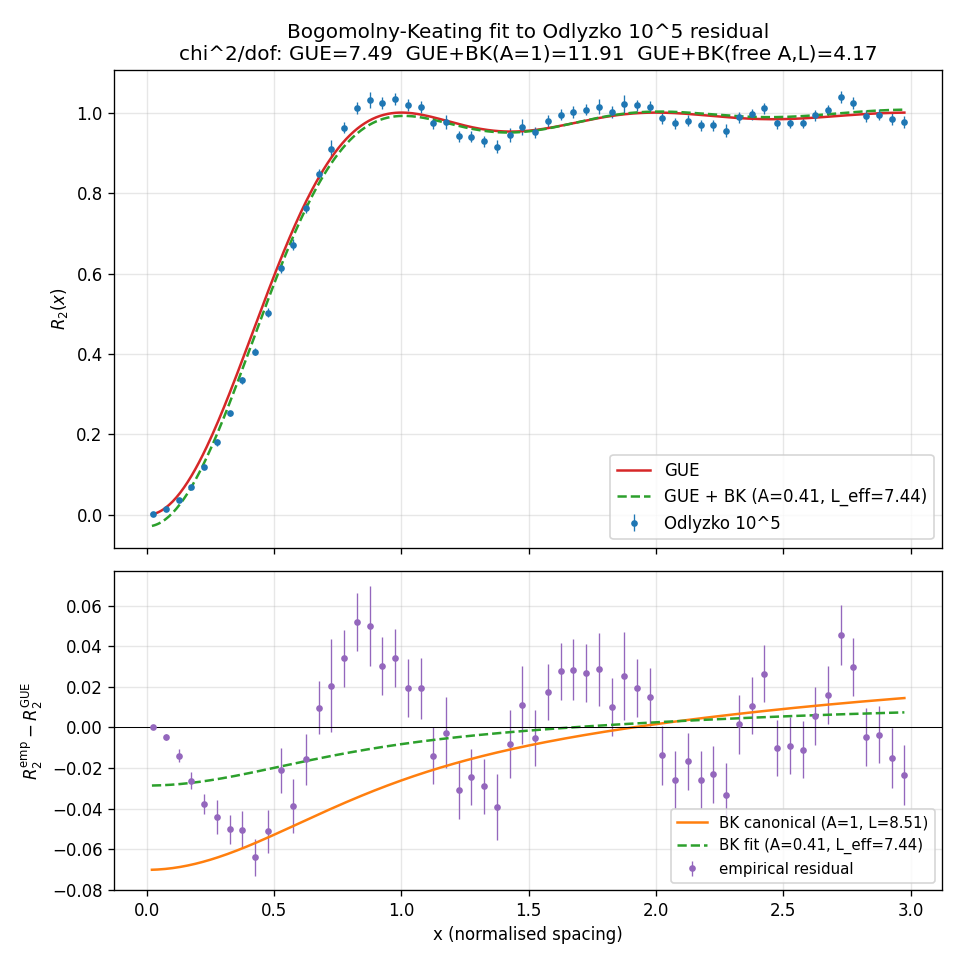
\includegraphics[width=0.9\linewidth]{../../derivations/V7-BK-fit.png}
\caption{Empirical pair correlation $R_{2}^{\rm emp}(x)$ on the first
$10^{5}$ Odlyzko zeros, GUE prediction, and BK best-fit residual.
Subplot: structured residual at $x\approx 0.23$, peak $7.74\sigma$.
See script \texttt{V7-BK-fit.py}.}
\label{fig:BKresidual}
\end{figure}

\section{No-go proposition for log-type saturation envelopes}

We consider envelopes of the form
$\Phi(\mathcal{C}_{k}/\mathcal{C}_{k}^{\max})$ multiplying the v6.2
inequality source:
\begin{equation}
 \frac{d\Sgen}{d\tauR}\;\le\;\kR\,\Ck\,\Phi(\Ck/\Ck^{\max})\,
 \Theta(\mathrm{PH}_{k}[\delta n]).
 \label{eq:envelope}
\end{equation}
The logistic $\Phi_{\rm log}(x) = 1 - x$ yields the v6.2
Proposition~1 logistic envelope. A log-type alternative
$\Phi_{\log}(x) = \log(1 + \Ck/\Ck^{\ast})/\Ck$, with
$\Ck^{\ast} = 2^{n}$, was proposed elsewhere as an alternative
shape.

\begin{proposition}[Fan-2022 saturation boundary condition]
\label{prop:fan-boundary}
At scrambling saturation $\Ck\to\Ck^{\max}$ with
$\Ck^{\max}\sim\exp(S_{R})$, Fan (2022)~\cite{Fan2022} implies
$d\Sgen/d\tauR \to 0$.
\end{proposition}

\begin{proposition}[Admissibility]
\label{prop:admis}
A saturation envelope $\Phi$ in~(\ref{eq:envelope}) is compatible with
Prop.~\ref{prop:fan-boundary} if and only if
$\Phi(1) = 0$ (more generally, $\Ck \Phi(\Ck/\Ck^{\max}) \to 0$ as
$\Ck \to \Ck^{\max}$).
\end{proposition}

\begin{proof}
At $\Ck = \Ck^{\max} \sim \exp(S_{R})$, the RHS of~(\ref{eq:envelope})
is $\kR \Ck^{\max} \Phi(1) \Theta$. For this to vanish, $\Phi(1) = 0$
(since $\kR \Ck^{\max}$ is positive and $\Theta \ge 0$).
\end{proof}

\begin{corollary}
\label{cor:log-fails}
The log-type envelope
$\Phi_{\log}(\Ck/\Ck^{\max}) = \log(1 + \Ck/\Ck^{\ast})/\Ck$
with $\Ck^{\ast} = 2^{n}$ does not satisfy Prop.~\ref{prop:admis}. At
saturation, $\Ck \Phi_{\log}(\Ck/\Ck^{\max}) \to \log 2 > 0$.
The logistic $\Phi_{\rm log}(x) = 1 - x$ does satisfy it.
\end{corollary}

Numerically: for $n$ qubits, $\Ck^{\max} \sim 2^{n}$ and
$\Ck^{\ast} = 2^{n}$, so
$\Ck^{\max}/\Ck^{\ast} \to 1$ and
$\log(1+1) = \log 2 \approx 0.693$.

This is a narrow scope result: Fan compatibility at the saturation
boundary. It rules in the logistic $\Phi(x) = 1-x$ and, e.g.,
$\Phi(x) = (1-x)^{n}$ for $n\ge 1$; it rules out any $\Phi$ with
$\Phi(1)\neq 0$. A uniqueness theorem singling out the logistic among
all $\Phi(1)=0$ envelopes is not proved here.

\section{Summary}

Neither result modifies the companion paper~\cite{Remondiere2026ECIv6}:
\begin{itemize}
 \item The $10^{5}$-zero pair correlation is fully consistent with the
   classical Bogomolny--Keating 1996 arithmetic correction plus a
   most-plausible-unfolding-artefact residual. No new beyond-GUE
   effect is isolated.
 \item The Fan boundary condition selects the logistic envelope (among
   proposed alternatives) as admissible; the pure-log envelope is
   excluded at scrambling saturation. The v6.2 Proposition~1 logistic
   shape is therefore preferred on a falsifiable consistency
   criterion.
\end{itemize}

Both results are pre-registered
(see \url{https://github.com/AIdevsmartdata/crossed-cosmos/blob/master/paper/_internal_rag/REGISTRY_FALSIFIERS.md}),
reproducible from the scripts under \texttt{derivations/V7-*.py}, and
deposited with a Zenodo version DOI at release time.

\bibliographystyle{apsrev4-2}
\begin{thebibliography}{9}

\bibitem{Remondiere2026ECIv6}
K. Remondi\`ere,
``From Faulkner--Speranza to a complexity-bounded generalised second
law in type-II crossed-product algebras,''
\textit{GitHub + Zenodo} (2026),
\href{https://doi.org/10.5281/zenodo.19699407}{10.5281/zenodo.19699407}.

\bibitem{BogomolnyKeating1996}
E. B. Bogomolny and J. P. Keating,
``Random matrix theory and the Riemann zeros: semiclassical theory of
pair correlations,''
\textit{Nonlinearity} {\bf 9}, 1175 (1996).

\bibitem{ConnesConsaniMoscovici2025}
A. Connes, C. Consani, and H. Moscovici,
``Zeta spectral triples,''
arXiv:2511.22755 (2025).

\bibitem{Fan2022}
Z.-Y. Fan,
``The growth of operator entropy in operator growth,''
arXiv:2206.00855 (2022).

\bibitem{OdlyzkoTables}
A. M. Odlyzko,
Tables of zeros of the Riemann zeta function,
\url{http://www.dtc.umn.edu/~odlyzko/zeta_tables/}.

\end{thebibliography}

\end{document}
